\documentclass{beamer}
\usepackage[polish,british]{babel}
\usepackage[utf8]{inputenc}
\usepackage{enumerate}

\author{Paweł Paczuski\\ \texttt{p.paczuski@stud.elka.pw.edu.pl}}
\title{Structured reporting system}
\date{06.04.2018}
\begin{document}
\begin{frame}
\titlepage
\end{frame}

\section*{Outline}
\begin{frame}
\frametitle{Outline}
\tableofcontents
\end{frame}

\section{Introduction}
\subsection{Problems of modern medicine}
\begin{frame}
\frametitle{Areas of interest of modern medicine}
\begin{itemize}
	\item increasing variety of diagnostic techniques and procedures
	\item unsatisfiable demand for medical services
	\item bureaucracy
	\item huge volumes of data to process and store. \alert{Healthcare Informatics}
\end{itemize}
\end{frame}

\begin{frame}
\frametitle{Healthcare Informatics vs Computer Science}
\end{frame}

\subsection{Standards}
\begin{frame}
\frametitle{Healthcare standards}
\begin{itemize}
	\item medical nomenclature SNOMED CT, LOINC
	\item exchange protocols and formats HL7, DICOM
\end{itemize}
\end{frame}

\subsection{Typical workflow of a radiologist}
\begin{frame}
\frametitle{Typical workflow of a radiologist}
\begin{figure}
	\centering
	\includegraphics[width=1\linewidth]{../workspace}
	\caption{Typically, a radiologist analyzes medical images and creates report's text simultaneously}
	\label{fig:workspace}
\end{figure}
\end{frame}

\begin{frame}
\frametitle{Areas of optimization}
\begin{itemize}
	\item radiologists are \alert{very BAD} at typing on keyboard
	\item speech recognition has problems with capturing medical language
	\
\end{itemize}
\end{frame}

\section{Structured reporting system}



\section{}
\subsection{Radiological report as a tree}

\begin{frame}
\frametitle{Reporting ontology}
\begin{figure}
	\centering
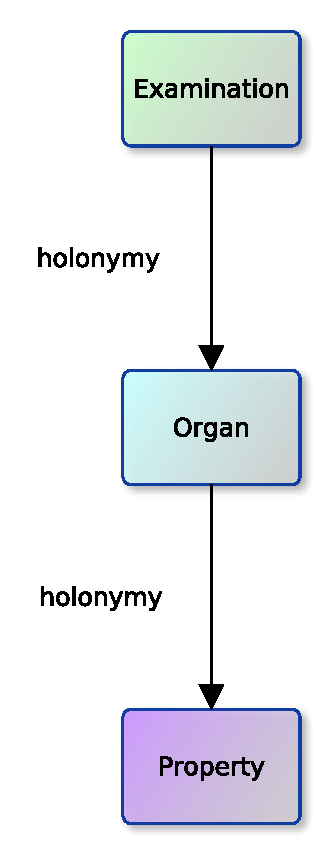
\includegraphics[width=0.2\linewidth]{../report-semantic}
\caption{Types of entities and relations between them}
\label{fig:report-ontology}
\end{figure}
\end{frame}


\begin{frame}
\frametitle{Radiological report as a tree}
\begin{figure}
	\centering
	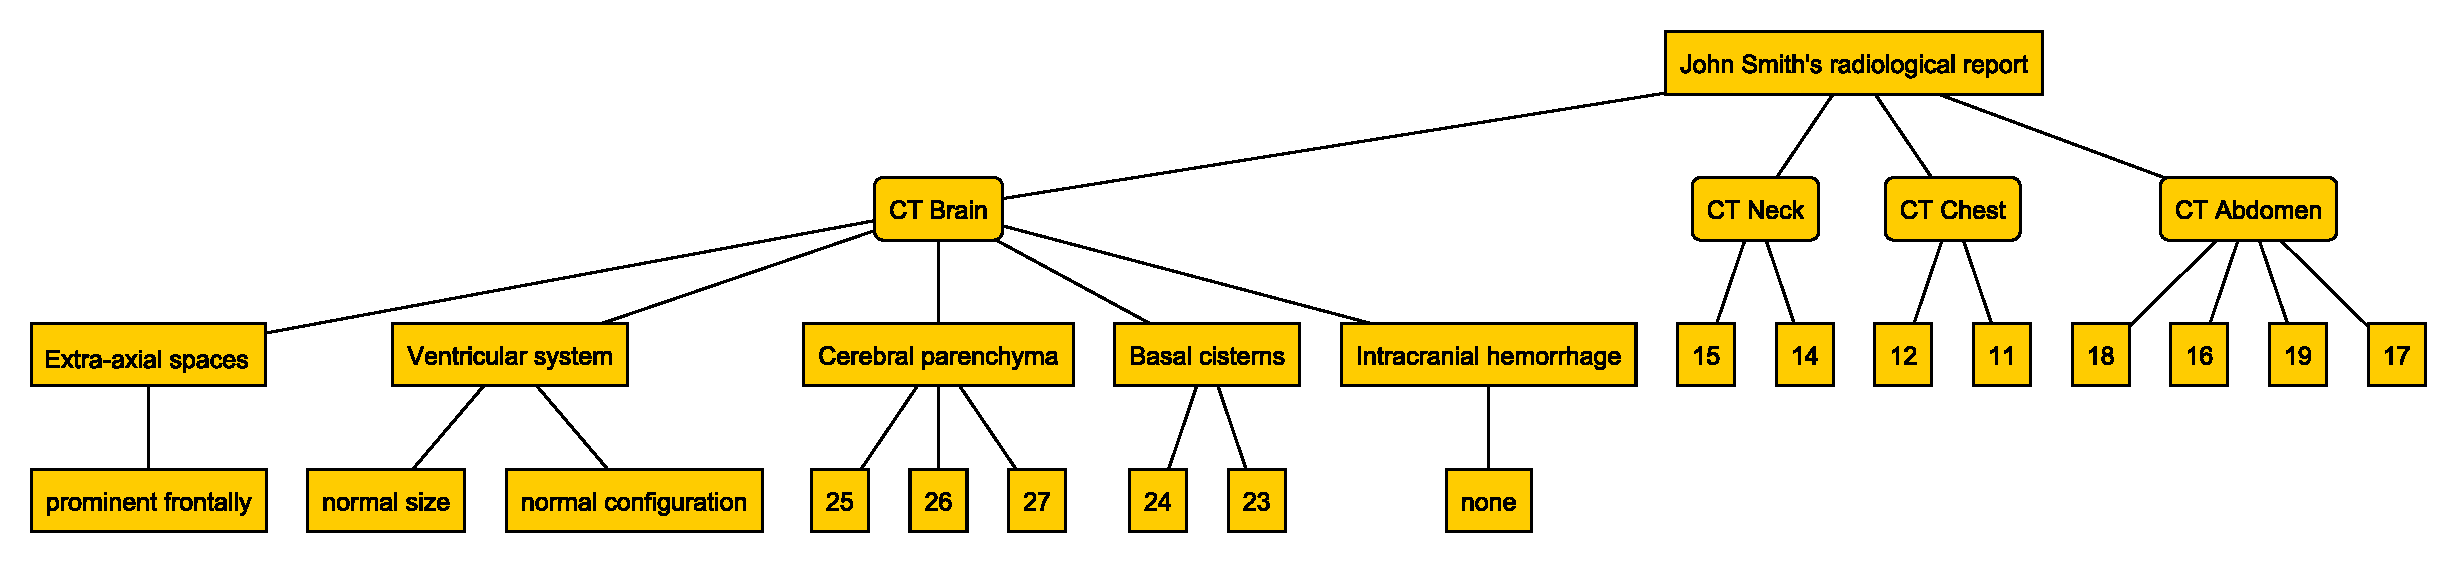
\includegraphics[width=1\linewidth]{../report-tree}
	\label{fig:report-tree}
\end{figure}
\end{frame}

\begin{frame}
\frametitle{Textual representation}
\begin{figure}
	\centering
	\includegraphics[width=1\linewidth]{../rendered-report}
	\label{fig:rendered-report}
\end{figure}
\end{frame}

\begin{frame}
\frametitle{Report editor interface}
\end{frame}







\end{document}
